\documentclass[a4paper,12pt,twocolumn,landscape]{article}

\usepackage{FabZ}
\usepackage{vecteurs}
\usepackage{repere}

\usepackage{geometry}
\geometry{hmargin=0.5cm,vmargin=1.5cm}

\newcommand{\milieu}[6]{$\pointcoord{A_{\theenumi}}{#1}{#2}$ et $\pointcoord{B_{\theenumi}}{#3}{#4}$ \hfill \reponseEX{$\pointcoord{M_{\theenumi}}{#5}{#6}$}}

\newcommand{\longueur}[5]{$\pointcoord{A_{\theenumi}}{#1}{#2}$ et $\pointcoord{B_{\theenumi}}{#3}{#4}$ \hfill \reponseEX{Longueur $A_{\theenumi}B_{\theenumi}$ = $#5$}}

\newcommand{\quadrilatere}[9]{$\pointcoord{A_{\theenumi}}{#1}{#2}$, $\pointcoord{B_\theenumi}{#3}{#4}$ $\pointcoord{C_{\theenumi}}{#5}{#6}$, $\pointcoord{D_\theenumi}{#7}{#8}$ \\ \textcolor{red}{$A_{\theenumi}B_{\theenumi}C_{\theenumi}D_{\theenumi}$ est un #9.}}

%\setlength{\headheight}{0pt}
%\pagestyle{fancyplain}
%\fancyhf{}
%\lhead[]{\textbf{TD Vecteurs}}
%\chead[]{}
%\rhead[]{}
%
%\lfoot[]{}
%\cfoot[]{}
%\rfoot[]{}
%%\rfoot[]{Page \thepage~ sur \pageref{LastPage}}

\fancypagestyle{firststyle}
{
	\setlength{\headheight}{0em}
	\fancyhf{}
	\lhead[]{\textbf{Repérage dans le plan}}
	\chead[]{}
	\rhead[]{\textbf{Repérage dans le plan}}

	\lfoot[]{}
	\cfoot[]{}
	\rfoot[]{}
%	\rfoot[]{Page \thepage~ sur \pageref{LastPage}}
}

\fancypagestyle{vide}
{
	\setlength{\headheight}{0em}
	\pagestyle{fancyplain}
	\def\headrulewidth{0em}
	\fancyhf{}
	\lhead[]{}
	\chead[]{}
	\rhead[]{}
	
	\lfoot[]{}
	\cfoot[]{}
	\rfoot[]{}
%	\rfoot[]{Page \thepage~ sur \pageref{LastPage}}
}

\usetikzlibrary{fadings}
\newcommand{\Fin}{node[xshift=-1.5ex,rotate=10]{F}
node[rotate=170]{i}
node[xshift=1.5ex,rotate=45]{n}}

\newcommand{\bonnesvacances}{node[xshift=0ex,rotate=10]{B}
node[xshift=1*1.5ex,rotate=170]{o}
node[xshift=2*1.5ex,rotate=45]{n}
node[xshift=3*1.5ex,rotate=128]{n}
node[xshift=4*1.5ex,rotate=75]{e}
node[xshift=5*1.5ex,rotate=130]{s}
node[xshift=6*1.5ex,rotate=85]{~}
node[xshift=7*1.5ex,rotate=128]{v}
node[xshift=8*1.5ex,rotate=43]{a}
node[xshift=9*1.5ex,rotate=4]{c}
node[xshift=10*1.5ex,rotate=145]{a}
node[xshift=11*1.5ex,rotate=5]{n}
node[xshift=12*1.5ex,rotate=25]{c}
node[xshift=13*1.5ex,rotate=105]{e}
node[xshift=14*1.5ex,rotate=45]{s}
}


\begin{document}
\begin{minipage}{0.45\textwidth}
\thispagestyle{firststyle}

\vspace*{1em}

\paragraph{Exercice~1} Donner les coordonnées des points dans les repères ci-dessous~:

\vspace{2em}

\begin{minipage}{0.7\textwidth}
		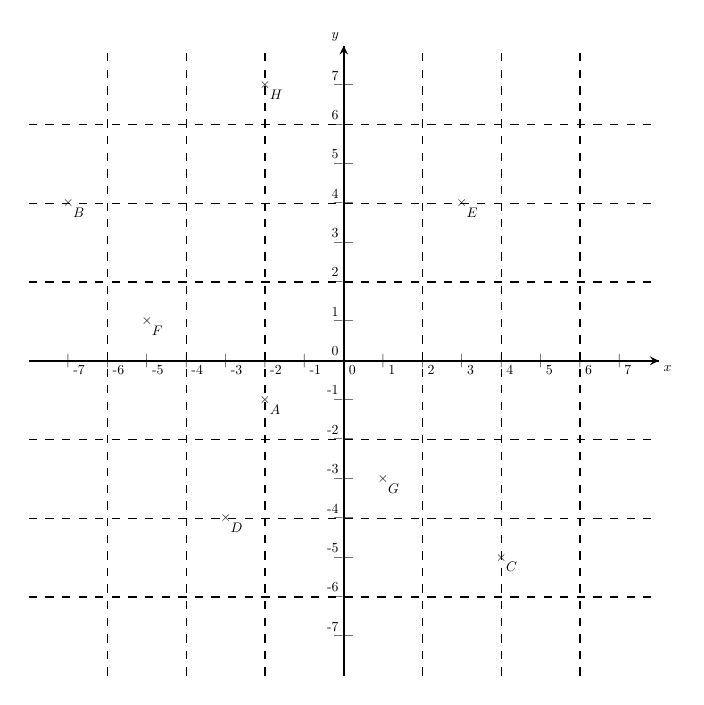
\begin{tikzpicture}[scale=0.5,every node/.style={scale=0.5}]
		%Points
		\coordinate(O)at(0,0);
		\coordinate(I)at(1,0);
		\coordinate(J)at(0,1);
		\coordinate(xstart)at(-8,0);
		\coordinate(xend)at(8,0);
		\coordinate(ystart)at(0,-8);
		\coordinate(yend)at(0,8);
		\coordinate(A)at(-2,-1);
		\coordinate(B)at(-7,4);
		\coordinate(C)at(4,-5);
		\coordinate(D)at(-3,-4);
		\coordinate(E)at(3,4);
		\coordinate(F)at(-5,1);
		\coordinate(G)at(1,-3);
		\coordinate(H)at(-2,7);
		%Étiquettes
	%	\draw (I) node[below right] {$1$};
	%	\draw (J) node[above left] {$1$};
		\draw (xend) node[below right] {$x$};
		\draw (yend) node[above left] {$y$};	
		%%%%%%%%%%%%%%%%%%%%%%%%%%%%%%%%%%%%
		%Axes
		\draw [thick] (xstart) -- (xend);
		\draw [thick] (ystart) -- (yend);
		%Flèches
	%	\draw [>=stealth,->] (O) -- (I);
	%	\draw [>=stealth,->] (O) -- (J);
		\draw [>=stealth,->] (O) -- (xend);
		\draw [>=stealth,->] (O) -- (yend);
	%	%Grille
	%	\draw [thin] (-8,-8)grid(8,8);
		%%%%%%%%%%%%%%%%%%%%%%%%%%%%%%%%%%%%
		%étiquettes
		\foreach \point in {A, ..., H}
			\draw(\point)node{$\times$};
		\foreach \point in {A, ..., H}
			\draw(\point)node[below right]{$\point$};		
		\foreach \r in {-7, -6, ..., 7}
	    	\draw[thick, below right] (\r,0) node{\r};
		\foreach \r in {-7, -6, ..., 7}
	    	\draw[thick, above left] (0,\r) node{\r};  
		\foreach \r in {-7, -6, ..., 7}
	    	\draw[thick] (\r,0) node{$|$};
		\foreach \r in {-7, -6, ..., 7}
	    	\draw[thick] (0,\r) node{$--$};
	   	\foreach \r in {-6, -4, ..., 6}
	    	\draw[dashed] (-8,\r)--(8,\r);
	   	\foreach \r in {-6, -4, ..., 6}
	    	\draw[dashed] (\r,-8)--(\r,8);
	%	\foreach \r in {0, 1,...,7}
	%    	\draw[thick, below right] (\r,0) node{\r};
	\end{tikzpicture}

\end{minipage}
\begin{minipage}{0.2\textwidth}
	\begin{enumerate}[]
		\item $\pointcoord{A}{~~~~}{~~~~}$
		\item $\pointcoord{B}{~~~~}{~~~~}$
		\item $\pointcoord{C}{~~~~}{~~~~}$
		\item $\pointcoord{D}{~~~~}{~~~~}$
		\item $\pointcoord{E}{~~~~}{~~~~}$
		\item $\pointcoord{F}{~~~~}{~~~~}$
		\item $\pointcoord{G}{~~~~}{~~~~}$
		\item $\pointcoord{H}{~~~~}{~~~~}$
	\end{enumerate}
\end{minipage}

\vspace{2em}

\begin{minipage}{0.7\textwidth}
				\begin{tikzpicture}[line cap=round,line join=round,>=triangle 45,x=1.0cm,y=1.0cm,scale=1,every node/.style={scale=1}]
			
			\tikzstyle{tiret}=[dash pattern=on 3pt off 3pt];
			\tikzstyle{domaine}=[domain=-5:8];
			\clip(-3.5,-2.5) rectangle (5.5,2.5);
			\draw [domaine] plot(\x,{(-0-0*\x)/1});
			\draw [domaine] plot(\x,{(-0--1*\x)/1});
			\draw [tiret,domaine] plot(\x,{(-1--1*\x)/1});
			\draw [tiret,domaine] plot(\x,{(-2--1*\x)/1});
			\draw [tiret,domaine] plot(\x,{(-3--1*\x)/1});
			\draw [tiret,domaine] plot(\x,{(-4--1*\x)/1});
			\draw [tiret,domaine] plot(\x,{(-5--1*\x)/1});
			\draw [tiret,domaine] plot(\x,{(--1--1*\x)/1});
			\draw [tiret,domaine] plot(\x,{(--2--1*\x)/1});
			\draw [tiret,domaine] plot(\x,{(--3--1*\x)/1});
			\draw [tiret,domaine] plot(\x,{(--1-0*\x)/1});
			\draw [tiret,domaine] plot(\x,{(--2-0*\x)/1});
			\draw [tiret,domaine] plot(\x,{(-1-0*\x)/1});
			\draw [tiret,domaine] plot(\x,{(-2-0*\x)/1});
			\draw [tiret,domaine] plot(\x,{(--4--1*\x)/1});
			\draw [tiret,domaine] plot(\x,{(-6--1*\x)/1});
			\draw [domaine] plot(\x,{(-0-0*\x)/-1});
			\draw [domaine] plot(\x,{(-0-0*\x)/-1});
			\draw [domaine] plot(\x,{(-0-0*\x)/-1});
			\begin{scriptsize}
			\draw (0,0) node {$\times$} node[above left] {$A$};
			\draw (1,0) node {$\times$} node[above left] {$I$};
			\draw (1,1) node {$\times$} node[above left] {$J$};
			\draw (3,0) node {$\times$} node[above left] {$E$};
			\draw (5,2) node {$\times$} node[above left] {$F$};
			\draw (1,-1) node {$\times$} node[above left] {$D$};
			\draw (-2,-2) node {$\times$} node[above left] {$C$};
			\draw (-2,2) node {$\times$} node[above left] {$B$};
			\draw (-3,0) node {$\times$} node[above left] {$G$};
			\draw (-3,-1) node {$\times$} node[above left] {$H$};
			\end{scriptsize}
			\end{tikzpicture}

\end{minipage}
\begin{minipage}{0.2\textwidth}
	\begin{enumerate}[]
		\item $\pointcoord{A}{~~~~}{~~~~}$
		\item $\pointcoord{B}{~~~~}{~~~~}$
		\item $\pointcoord{C}{~~~~}{~~~~}$
		\item $\pointcoord{D}{~~~~}{~~~~}$
		\item $\pointcoord{E}{~~~~}{~~~~}$
		\item $\pointcoord{F}{~~~~}{~~~~}$
		\item $\pointcoord{G}{~~~~}{~~~~}$
		\item $\pointcoord{H}{~~~~}{~~~~}$
	\end{enumerate}
\end{minipage}


\vspace{-2em}

\end{minipage}
\newpage
\begin{minipage}{0.45\textwidth}
\thispagestyle{firststyle}

\vspace*{1em}

\paragraph{Exercice~1} Donner les coordonnées des points dans les repères ci-dessous~:

\vspace{2em}

\begin{minipage}{0.7\textwidth}
		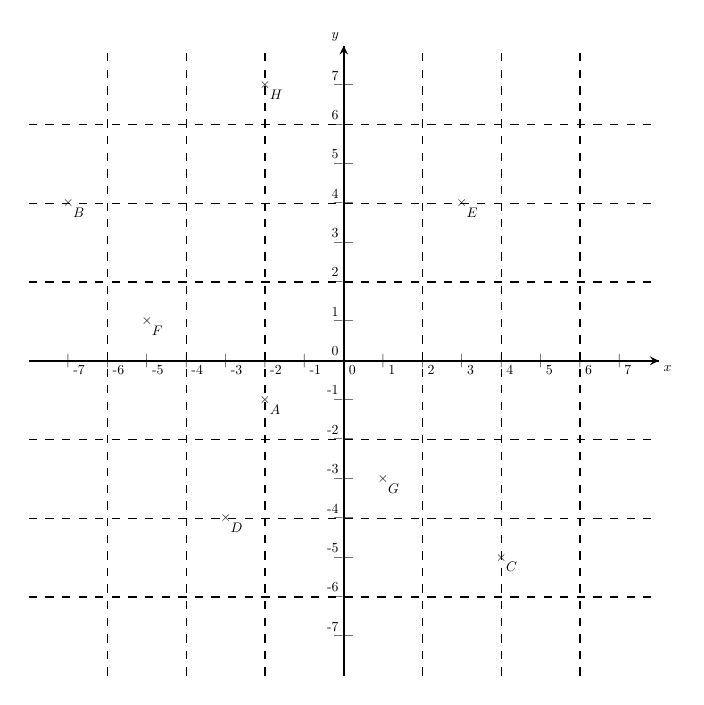
\begin{tikzpicture}[scale=0.5,every node/.style={scale=0.5}]
		%Points
		\coordinate(O)at(0,0);
		\coordinate(I)at(1,0);
		\coordinate(J)at(0,1);
		\coordinate(xstart)at(-8,0);
		\coordinate(xend)at(8,0);
		\coordinate(ystart)at(0,-8);
		\coordinate(yend)at(0,8);
		\coordinate(A)at(-2,-1);
		\coordinate(B)at(-7,4);
		\coordinate(C)at(4,-5);
		\coordinate(D)at(-3,-4);
		\coordinate(E)at(3,4);
		\coordinate(F)at(-5,1);
		\coordinate(G)at(1,-3);
		\coordinate(H)at(-2,7);
		%Étiquettes
	%	\draw (I) node[below right] {$1$};
	%	\draw (J) node[above left] {$1$};
		\draw (xend) node[below right] {$x$};
		\draw (yend) node[above left] {$y$};	
		%%%%%%%%%%%%%%%%%%%%%%%%%%%%%%%%%%%%
		%Axes
		\draw [thick] (xstart) -- (xend);
		\draw [thick] (ystart) -- (yend);
		%Flèches
	%	\draw [>=stealth,->] (O) -- (I);
	%	\draw [>=stealth,->] (O) -- (J);
		\draw [>=stealth,->] (O) -- (xend);
		\draw [>=stealth,->] (O) -- (yend);
	%	%Grille
	%	\draw [thin] (-8,-8)grid(8,8);
		%%%%%%%%%%%%%%%%%%%%%%%%%%%%%%%%%%%%
		%étiquettes
		\foreach \point in {A, ..., H}
			\draw(\point)node{$\times$};
		\foreach \point in {A, ..., H}
			\draw(\point)node[below right]{$\point$};		
		\foreach \r in {-7, -6, ..., 7}
	    	\draw[thick, below right] (\r,0) node{\r};
		\foreach \r in {-7, -6, ..., 7}
	    	\draw[thick, above left] (0,\r) node{\r};  
		\foreach \r in {-7, -6, ..., 7}
	    	\draw[thick] (\r,0) node{$|$};
		\foreach \r in {-7, -6, ..., 7}
	    	\draw[thick] (0,\r) node{$--$};
	   	\foreach \r in {-6, -4, ..., 6}
	    	\draw[dashed] (-8,\r)--(8,\r);
	   	\foreach \r in {-6, -4, ..., 6}
	    	\draw[dashed] (\r,-8)--(\r,8);
	%	\foreach \r in {0, 1,...,7}
	%    	\draw[thick, below right] (\r,0) node{\r};
	\end{tikzpicture}

\end{minipage}
\begin{minipage}{0.2\textwidth}
	\begin{enumerate}[]
		\item $\pointcoord{A}{~~~~}{~~~~}$
		\item $\pointcoord{B}{~~~~}{~~~~}$
		\item $\pointcoord{C}{~~~~}{~~~~}$
		\item $\pointcoord{D}{~~~~}{~~~~}$
		\item $\pointcoord{E}{~~~~}{~~~~}$
		\item $\pointcoord{F}{~~~~}{~~~~}$
		\item $\pointcoord{G}{~~~~}{~~~~}$
		\item $\pointcoord{H}{~~~~}{~~~~}$
	\end{enumerate}
\end{minipage}

\vspace{2em}

\begin{minipage}{0.7\textwidth}
				\begin{tikzpicture}[line cap=round,line join=round,>=triangle 45,x=1.0cm,y=1.0cm,scale=1,every node/.style={scale=1}]
			
			\tikzstyle{tiret}=[dash pattern=on 3pt off 3pt];
			\tikzstyle{domaine}=[domain=-5:8];
			\clip(-3.5,-2.5) rectangle (5.5,2.5);
			\draw [domaine] plot(\x,{(-0-0*\x)/1});
			\draw [domaine] plot(\x,{(-0--1*\x)/1});
			\draw [tiret,domaine] plot(\x,{(-1--1*\x)/1});
			\draw [tiret,domaine] plot(\x,{(-2--1*\x)/1});
			\draw [tiret,domaine] plot(\x,{(-3--1*\x)/1});
			\draw [tiret,domaine] plot(\x,{(-4--1*\x)/1});
			\draw [tiret,domaine] plot(\x,{(-5--1*\x)/1});
			\draw [tiret,domaine] plot(\x,{(--1--1*\x)/1});
			\draw [tiret,domaine] plot(\x,{(--2--1*\x)/1});
			\draw [tiret,domaine] plot(\x,{(--3--1*\x)/1});
			\draw [tiret,domaine] plot(\x,{(--1-0*\x)/1});
			\draw [tiret,domaine] plot(\x,{(--2-0*\x)/1});
			\draw [tiret,domaine] plot(\x,{(-1-0*\x)/1});
			\draw [tiret,domaine] plot(\x,{(-2-0*\x)/1});
			\draw [tiret,domaine] plot(\x,{(--4--1*\x)/1});
			\draw [tiret,domaine] plot(\x,{(-6--1*\x)/1});
			\draw [domaine] plot(\x,{(-0-0*\x)/-1});
			\draw [domaine] plot(\x,{(-0-0*\x)/-1});
			\draw [domaine] plot(\x,{(-0-0*\x)/-1});
			\begin{scriptsize}
			\draw (0,0) node {$\times$} node[above left] {$A$};
			\draw (1,0) node {$\times$} node[above left] {$I$};
			\draw (1,1) node {$\times$} node[above left] {$J$};
			\draw (3,0) node {$\times$} node[above left] {$E$};
			\draw (5,2) node {$\times$} node[above left] {$F$};
			\draw (1,-1) node {$\times$} node[above left] {$D$};
			\draw (-2,-2) node {$\times$} node[above left] {$C$};
			\draw (-2,2) node {$\times$} node[above left] {$B$};
			\draw (-3,0) node {$\times$} node[above left] {$G$};
			\draw (-3,-1) node {$\times$} node[above left] {$H$};
			\end{scriptsize}
			\end{tikzpicture}

\end{minipage}
\begin{minipage}{0.2\textwidth}
	\begin{enumerate}[]
		\item $\pointcoord{A}{~~~~}{~~~~}$
		\item $\pointcoord{B}{~~~~}{~~~~}$
		\item $\pointcoord{C}{~~~~}{~~~~}$
		\item $\pointcoord{D}{~~~~}{~~~~}$
		\item $\pointcoord{E}{~~~~}{~~~~}$
		\item $\pointcoord{F}{~~~~}{~~~~}$
		\item $\pointcoord{G}{~~~~}{~~~~}$
		\item $\pointcoord{H}{~~~~}{~~~~}$
	\end{enumerate}
\end{minipage}


\vspace{-2em}

\end{minipage}
\end{document}
%
%
%\paragraph{Exercice~2} Propriétés des quadrilatères
%
%\begin{tikzpicture}[scale=1,every node/.style={scale=0.7}]
%\tikzstyle{debutfin}=[ellipse,draw,text=red]
%\tikzstyle{instruct}=[rectangle,draw,fill=yellow!50]
%\tikzstyle{test}=[diamond, aspect=6,thick,
%draw=blue,fill=yellow!50,text=blue]
%\tikzstyle{es}=[rectangle,draw,rounded corners=4pt,fill=blue!25]
%
%\node[debutfin] (debut) at (0,3) {Début};
%\node[es] (lire) at (0,2) {Prendre un quadrilatère $Q$};
%\node[test] (test) at (0,0) {Les diagonales ont-elles un milieu commun \ ?};
%%\node[instruct] (init) at (-2,2.5) {$S\leftarrow 0$};
%\node[instruct] (plus) at (0,-2.5) {$S\leftarrow S+N$};
%\node[instruct] (moins) at (0,-3.5) {$N\leftarrow N-1$};
%\node[es] (afficher) at (-4,-2) {Afficher la somme $S$};
%\node[debutfin] (fin) at (-4,-3) {Fin};
%
%\tikzstyle{suite}=[->,>=stealth,thick,rounded corners=4pt]
%\draw[suite](debut) -- (lire);
%\draw[suite](lire) -- (test.north);
%%\draw[suite](init) -- (test.north);
%\draw[suite](test.south) -- (plus);
%\draw[suite](plus) -- (moins);
%\draw[suite](test) -| (afficher);
%\draw[suite](afficher) -- (fin);
%\end{tikzpicture}
%
%
%%%%%\begin{tikzpicture}
%%%%%% définition des styles
%%%%%\tikzstyle{quadri}=[rectangle,draw,fill=yellow!50,text=blue]
%%%%%\tikzstyle{estun}=[->,>=latex,very thick,dotted]
%%%%%% les nœuds
%%%%%\node[quadri] (Q) at (0,3) {Quadrilatère};
%%%%%\node[quadri] (P) at (0,1.5) {Parallélogramme};
%%%%%\node[quadri] (R) at (-3,0) {Rectangle};
%%%%%\node[quadri] (L) at (3,0) {Losange};
%%%%%\node[quadri] (C) at (5,-1.5) {Carré};
%%%%%% les flèches
%%%%%\draw[estun] (P)--(Q);
%%%%%\draw[estun] (R)to[bend left](Q); \draw[estun] (R)--(P);
%%%%%\draw[estun] (L)--(Q.south east); \draw[estun] (L)--(P);
%%%%%\draw[estun] (C)to[bend right](Q.east); \draw[estun] (C)to[bend left](P);
%%%%%\draw[estun] (C)--(L.south east); \draw[estun] (C)to[bend left](R);
%%%%%% la légende
%%%%%\draw[estun] (-4.5,2.5)--(-3,2.5)node[midway,above]{est un};
%%%%%\end{tikzpicture}